\chapter{Application}
In this chapter, the data is analyzed for cointegration. First, it will be done pairwise using Engle Granger. Secondly, it will be tested for all four simultaneously with the use of the Johansen test. After the models are build they will be used for forecasting, where the predictions will be compared to the validation data, to test the precision of the models.


\section{Engle Granger Model Building}
To build the models, we first check for cointegration. This is done by making a linear model of all the $12$ possible combinations of the cryptocurrencies. In theory, cointegration is not directional, but in practice one acts as the regressand, and therefore we check all $12$ combinations. From this test, four models gave a $p$-value that rejected the null hypothesis, meaning they were stationary, but to check if they are cointegrated, one must check if their critical value is larger than the given test statistic for the model. An example of this is shown for Solana and Ethereum, here the histogram, ACF, and residual plot are made to check for constant and trend. This is because the critical value changes depending on whether the data includes a trend or a constant, as determined by the augmented Dickey-Fuller test. 
\begin{figure}[h]
    \centering
    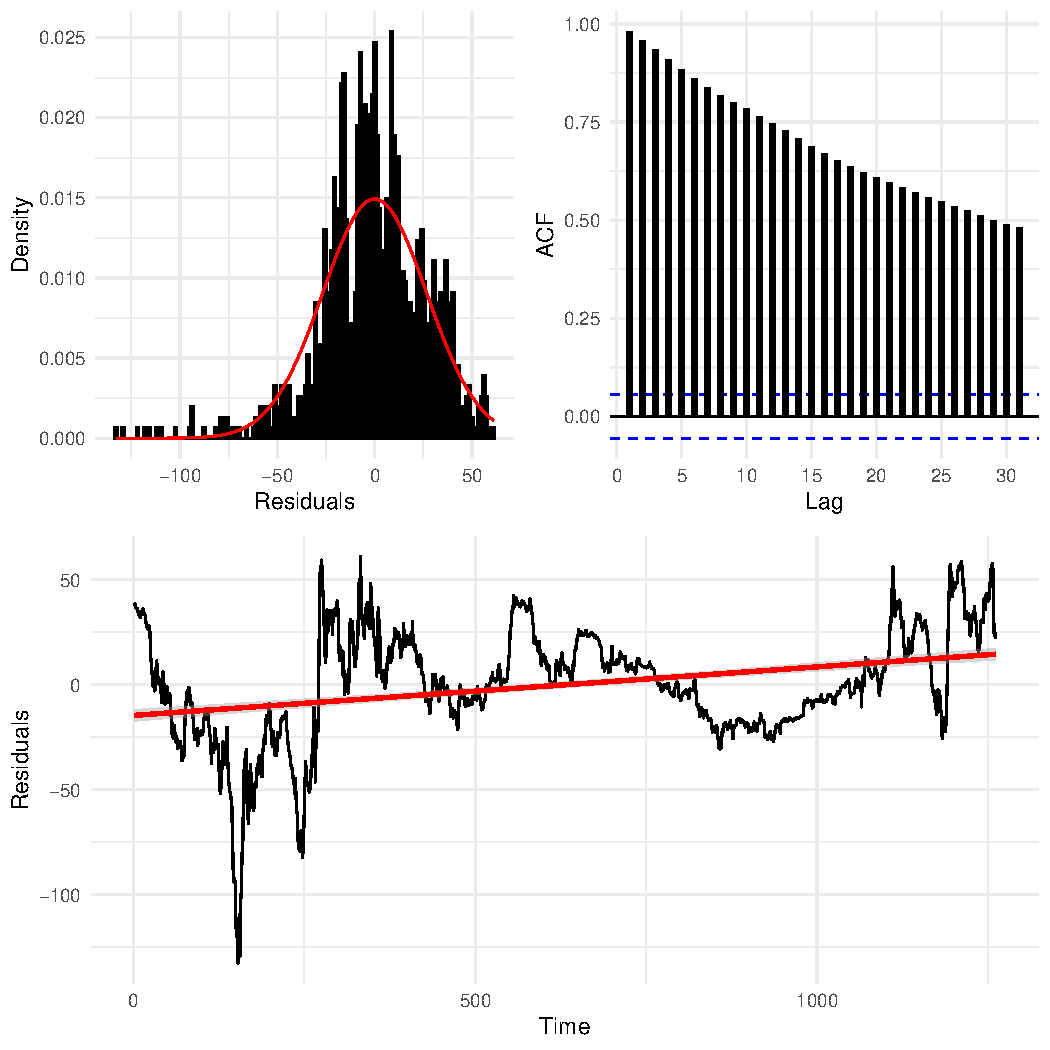
\includegraphics[width=0.4\linewidth]{1.Projekt_kode/Billeder/plot_grid_ADF_Solana-Ethereum.pdf}
    \caption{Residuals of Solana and Ethereum model}
    \label{fig:ADF_HIST_GRAPH_SOLANA_ETHEREUM}
\end{figure}

\noindent In Figure \ref{fig:ADF_HIST_GRAPH_SOLANA_ETHEREUM}, it is evident from the ACF plot that trend is present in the data, but there are no indication of a constant in the model. When this is the case, the critical value is $-3.413$ (see \cite{ADf_crit_val}). As the critical value is greater than the test statistic, the null hypothesis is rejected, confirming that the data indicates stationarity. \\
\noindent This procedure is repeated for the three other models, all of which also rejects the null hypothesis. 


\pause
\begin{center}
\begin{tabular}{cccc}
   Solana \& Ethereum \quad & \quad Ripple \& Ethereum\\\\
   Ethereum \& Solana \quad & \quad Ripple \& Solana
\end{tabular}
\end{center}
\pause
\noindent The four cases will be abbreviated as SOL\&ETH, XRP\&ETH, ETH\&SOL, and XRP\&SOL. Next, a VECM will be constructed in the instances, where the ADF test indicates cointegration in both directions. This is because the cases where cointegration was found, but only in one direction, a VECM cannot be constructed. For those cases an ECM could be build instead. This will however not be done, since we would have to forecast the predictor for the ECM using other means than cointegration. Therefore, the only model that will be considered is the SOL\&ETH, ETH\&SOL, since this will give us the same VECM model, only with a difference in the position of ETH and SOL. To proceed with the analysis, we need to determine the optimal lag order for the model. First, the R function \textit{VARselect} is used to find the optimal lag order. The AIC scores for the SOL\&ETH have been plotted in Figure \ref{fig:AIC_plots}. The optimal lag order for a VAR model for SOL\&ETH, is found by visual interpretation of Figure \ref{fig:AIC_plots}.
\begin{figure}[H]
  \centering
  \subfloat[][Solana \& Ethereum]{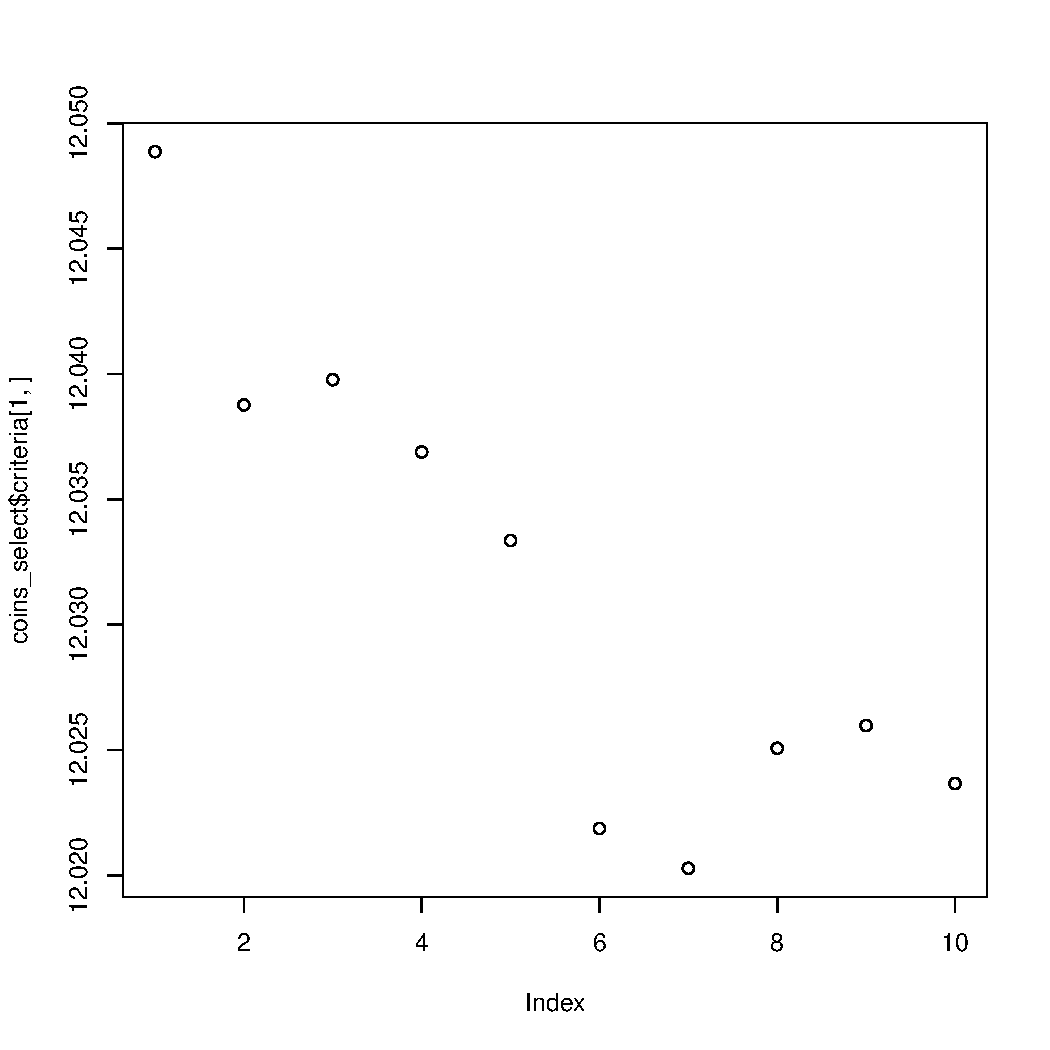
\includegraphics[width=.45\textwidth]{1.Projekt_kode/Billeder/AIC_Lag_forSolana_Ethereum.pdf}}\quad
  
  \caption{AIC values for SOL\&ETH}
  \label{fig:AIC_plots}
\end{figure}
\noindent The lag order is, from Figure \ref{fig:AIC_plots}, chosen to be seven. With the lag order determined, we are able to specify the VECM, where the lag order is $p-1$.

\noindent The VECM is specified as follows, represented as a system of equations:\\

\begin{center}
    \textbf{SOL \& ETH}
\end{center}
Here $\hat{\beta}$ is computed as $\hat{\beta} =[1, \quad -0.03250492 ]^\top$
\\
Equations:

\begin{align*}
\Delta \text{Solana}_t &= 
\underset{(0.0039)}{(-0.0066)} \cdot \text{ECT}_{t-1} + 
\underset{(0.1414)}{0.0657} + 
\underset{(0.0348)}{0.0413} \cdot \Delta \text{Solana}_{t-1} \\
&\quad + \underset{(0.0016)}{(-0.0024)} \cdot \Delta \text{Ethereum}_{t-1} + 
\underset{(0.0348)}{(-0.0166)} \cdot \Delta \text{Solana}_{t-2} \\
&\quad + \underset{(0.0016)}{0.0017} \cdot \Delta \text{Ethereum}_{t-2} + 
\underset{(0.0350)}{0.0403} \cdot \Delta \text{Solana}_{t-3} \\
&\quad + \underset{(0.0016)}{0.0019} \cdot \Delta \text{Ethereum}_{t-3} + 
\underset{(0.0349)}{0.0958} \cdot \Delta \text{Solana}_{t-4} \\
&\quad + \underset{(0.0017)}{(-0.0005)} \cdot \Delta \text{Ethereum}_{t-4} + 
\underset{(0.0351)}{(-0.0941)} \cdot \Delta \text{Solana}_{t-5} \\
&\quad + \underset{(0.0016)}{(-0.0009)} \cdot \Delta \text{Ethereum}_{t-5} + 
\underset{(0.0352)}{(-0.0497)} \cdot \Delta \text{Solana}_{t-6} \\
&\quad + \underset{(0.0016)}{0.0040} \cdot \Delta \text{Ethereum}_{t-6}.
\end{align*}

\begin{align*}
\Delta \text{Ethereum}_t &= 
\underset{(0.0830)}{(-0.0373)} \cdot \text{ECT}_{t-1} + 
\underset{(3.0208)}{2.2306} + 
\underset{(0.7446)}{(-1.5949)} \cdot \Delta \text{Solana}_{t-1} \\
&\quad + \underset{(0.0349)}{(-0.0267)} \cdot \Delta \text{Ethereum}_{t-1} + 
\underset{(0.7433)}{(-1.7485)} \cdot \Delta \text{Solana}_{t-2} \\
&\quad + \underset{(0.0348)}{0.0573} \cdot \Delta \text{Ethereum}_{t-2} + 
\underset{(0.7471)}{(-0.9073)} \cdot \Delta \text{Solana}_{t-3} \\
&\quad + \underset{(0.0349)}{0.0800} \cdot \Delta \text{Ethereum}_{t-3} + 
\underset{(0.7467)}{1.8720} \cdot \Delta \text{Solana}_{t-4} \\
&\quad + \underset{(0.0353)}{(-0.0123)} \cdot \Delta \text{Ethereum}_{t-4} + 
\underset{(0.7490)}{0.4281} \cdot \Delta \text{Solana}_{t-5} \\
&\quad + \underset{(0.0352)}{(-0.0668)} \cdot \Delta \text{Ethereum}_{t-5} + 
\underset{(0.7512)}{(-0.5645)} \cdot \Delta \text{Solana}_{t-6} \\
&\quad + \underset{(0.0350)}{0.0886} \cdot \Delta \text{Ethereum}_{t-6}.
\end{align*}

\section{Johansen Model Building}
One of the advantages, when using the Johansen test is its ability to detect cointegration among multiple time series at a time. This means that we are not restricted to analyzing pairwise integrated series. We will throughout this section use both the trace test statistic, explained in Section \cite{Johansen_test}, and the maximum eigenvalue test (which briefly will be described below). \\
The overall difference between the two tests is, that the trace test has $H_0$ stating, that there are at max $r$ cointegration relations, versus $H_1$ stating the presence of more than $r$ cointegration relations, and has the statistic given in \eqref{eq:lrmax_coint_r}. The maximum eigenvalue test has $H_0$ stating the presence of $r$ cointegration relations, whereas $H_1$ indicates the presence of $r+1$ cointegration relations, and has the statistic $-Tln(1-\hat{\lambda}_{r_0+1})$, meaning it tests each eigenvalue's influence individually.\\\\
Generally, there is little to no difference between the results achieved through the two tests. The trace test is more likely to dismiss $H_0$ even though it might be true, hence having higher probability of type 1 errors. At the same time, the trace test is more efficient in finding cointegration relations when they do exist and is more advantageous when multiple cointegration relations exist. Since both tests are beneficial in different scenarios, it is preferable to perform both to see whether they comply with each other, and if not, examine further why this could be the case \citep{johansentestdifferences}.



\subsection{Trace Test}\label{subsec:johansen_trace}
Using Johansen's trace test, a 5\% critical value is compared to the test statistic for $r=0,\;r\leq1,\;r\leq 2,\;r\leq3$.
The results are computed using the R function \textit{ca.jo} and shown below.
\begin{table}[H]
\centering
\begin{tabular}{|c|c|c|}
\hline
\textbf{Cointegration Relations} & \textbf{Test Statistic} & \textbf{5\% Critical Values} \\ \hline
$r \leq 3$ & 0.32  & 8.18  \\ \hline
$r \leq 2$ & 13.85 & 17.95 \\ \hline
$r \leq 1$ & 42.19 & 31.52 \\ \hline
$r = 0$    & 83.51 & 48.28 \\ \hline
\end{tabular}
\caption{Test statistics for Johansen trace test at 5\% significant level}
\label{tab:traceresults}
\end{table}
\noindent In Table \ref{tab:traceresults} it is seen that the test statistic for $r=0$ and $r\leq1$ are greater than the critical values. The corresponding null hypotheses are therefore rejected, and the hypothesis for $r\leq2$ cannot be rejected, since the test statistic is smaller than the critical value. This indicates the presence of two cointegration relations.

\subsection{Maximum Eigenvalue Test}
The maximum eigenvalue test is also used in order to see whether the two tests comply with each other. Once again the R function \textit{ca.jo} is used to compute the results and can be seen in Table \ref{tab:maximal_eigenvalue} where the setup is the same as for the trace test.
\begin{table}[H]
\centering
\begin{tabular}{|c|c|c|}
\hline
\textbf{Cointegration Relations} & \textbf{Test Statistic} & \textbf{5\% Critical Values} \\ \hline
$r \leq 3$ & 0.32  & 8.18  \\ \hline
$r \leq 2$ & 13.53 & 14.90 \\ \hline
$r \leq 1$ & 28.33 & 21.07 \\ \hline
$r = 0$    & 41.32 & 27.14 \\ \hline
\end{tabular}
\caption{Test statistics for Johansen maximum eigenvalue test at 5\% significant level}
\label{tab:maximal_eigenvalue}
\end{table}
\noindent Just as concluded in Section \ref{subsec:johansen_trace}, the maximum eigenvalue test also indicates two cointegration relations, and there are therefore no issues regarding contradictions in the tests.

\subsection{Model Choice}
After both the trace test and the maximum eigenvalue test suggest the presence of two cointegration relations, the next step is to apply the achieved conclusions in forecasting. The R function \textit{ca.jo} indicates that of the four eigenvalues only the two greatest, 0.0324140 and 0.0223421, are significant enough to indicate a cointegration relation.\\
Next, the R function \textit{cajorls} is used to fit a VECM with two cointegration relations. The error correction terms, hence the two $\beta$ vectors, are given in the table below:\\
\begin{table}[h!]
\centering
\begin{tabular}{|c|c|c|}
\hline
\textbf{Cryptocurrency} & $\hat{\b{\beta}}_1$ & $\hat{\b{\beta}}_2$ \\ \hline
 $\text{Bitcoin}_{t-7}$  & $1.00$  & $0.00$      \\ \hline
 $\text{Ethereum}_{t-7}$  & $-5.684342 \cdot 10^{-14}$ & $1.0000$    \\\hline
 $\text{Solana}_{t-7}$  & $-2.218088 \cdot 10^3$ & $-22.5305$    \\ \hline
 $\text{Ripple}_{t-7}$  & $1.248777 \cdot 10^6$  & $6121.3729$   \\ \hline
\end{tabular}
\caption{Johansen cointegration relations}
\label{tab:ect_coefficients}
\end{table}

\noindent Next, the VECM will be transformed into a VAR model, using the R function \textit{vec2var}, which will be used to forecast in the following section.



\section{Forecast}
To evaluate the models ability to forecast, we will first look at plots of a single 20-day-ahead prediction, where the predictions are plotted against the true values. Secondly, a five-day-ahead forecast, is made iteratively, with each iteration adding another day to the training set until the entire validation set is predicted. These predictions are evaluated using the three different accuracy measures, mean absolute value (MAE), root mean square error (RMSE), and mean absolute percentage error (MAPE). The MAE is straight forward, the RMSE gives more weight to outliers, and the MAPE is used because it intuitively gives a great understanding of the errors. The formulas for calculation is given below:
\begin{align*}
    \text{MAE} = \frac{1}{T} \sum_{i=1}^{T} |y_i - \hat{y}_i|, \quad \text{RMSE} = \sqrt{\frac{1}{T} \sum_{i=1}^{T} (y_i - \hat{y}_i)^2}, \quad \text{MAPE} = \frac{1}{T} \sum_{i=1}^{T} \left| \frac{y_i - \hat{y}_i}{y_i} \right|\cdot 100,
\end{align*}
\noindent where $y_i$ is the actual value, $\hat{y}_i$ is the predicted value, and $T$ is the number of observation.

\subsection{Engle Granger}\label{englegrangerforecastsection}
First the 20-day-ahead prediction plot will be examined. These predictions are however not very representable of the actual accuracy of the model, since it is just a single 20-day-ahead prediction. It does however, give an insight into whether the model is able to capture the movements of the actual data.
\begin{figure}[H]
  \centering
  \subfloat[][Solana]{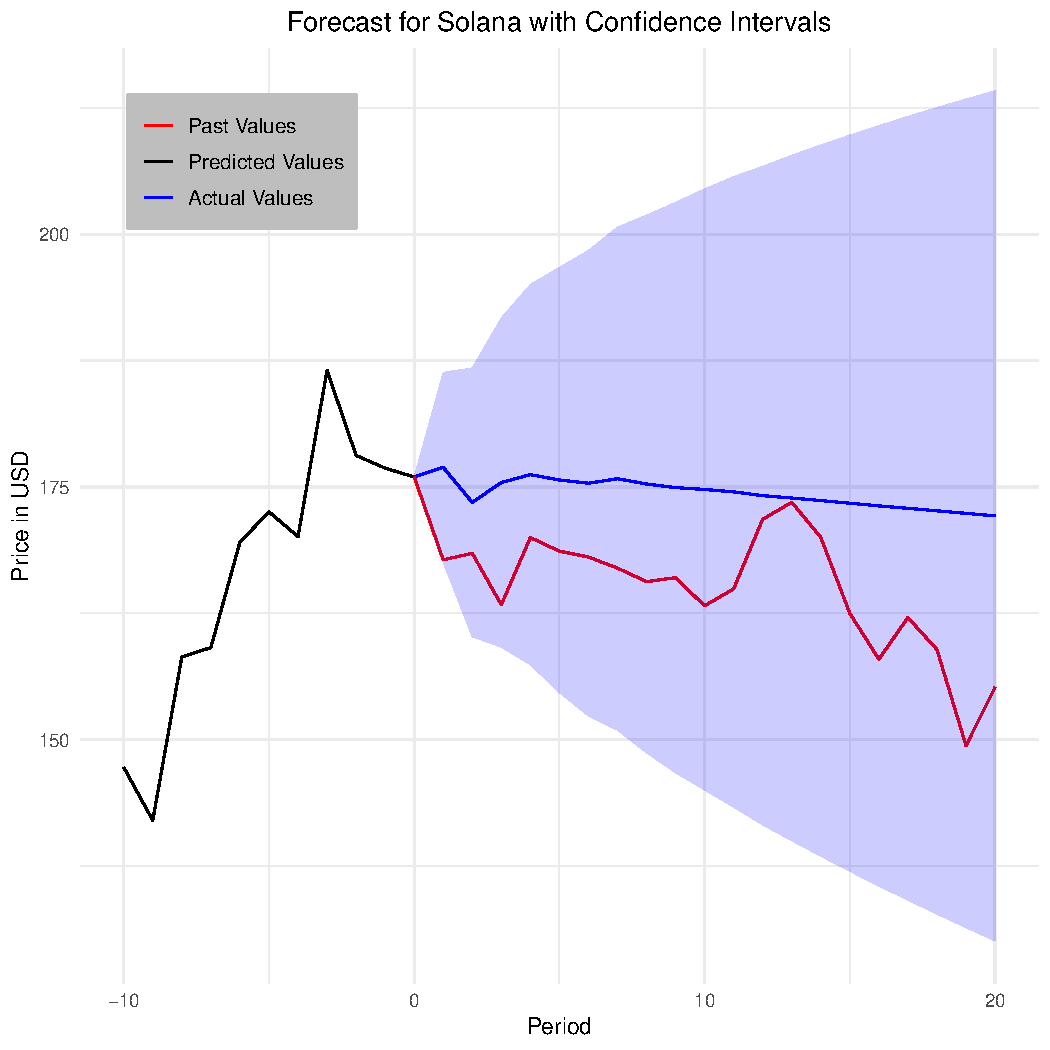
\includegraphics[width=.45\textwidth]{1.Projekt_kode/Billeder/20_day_ahed_Solana_from_Solana_Ethereum.pdf}}\quad
  \subfloat[][Ethereum]{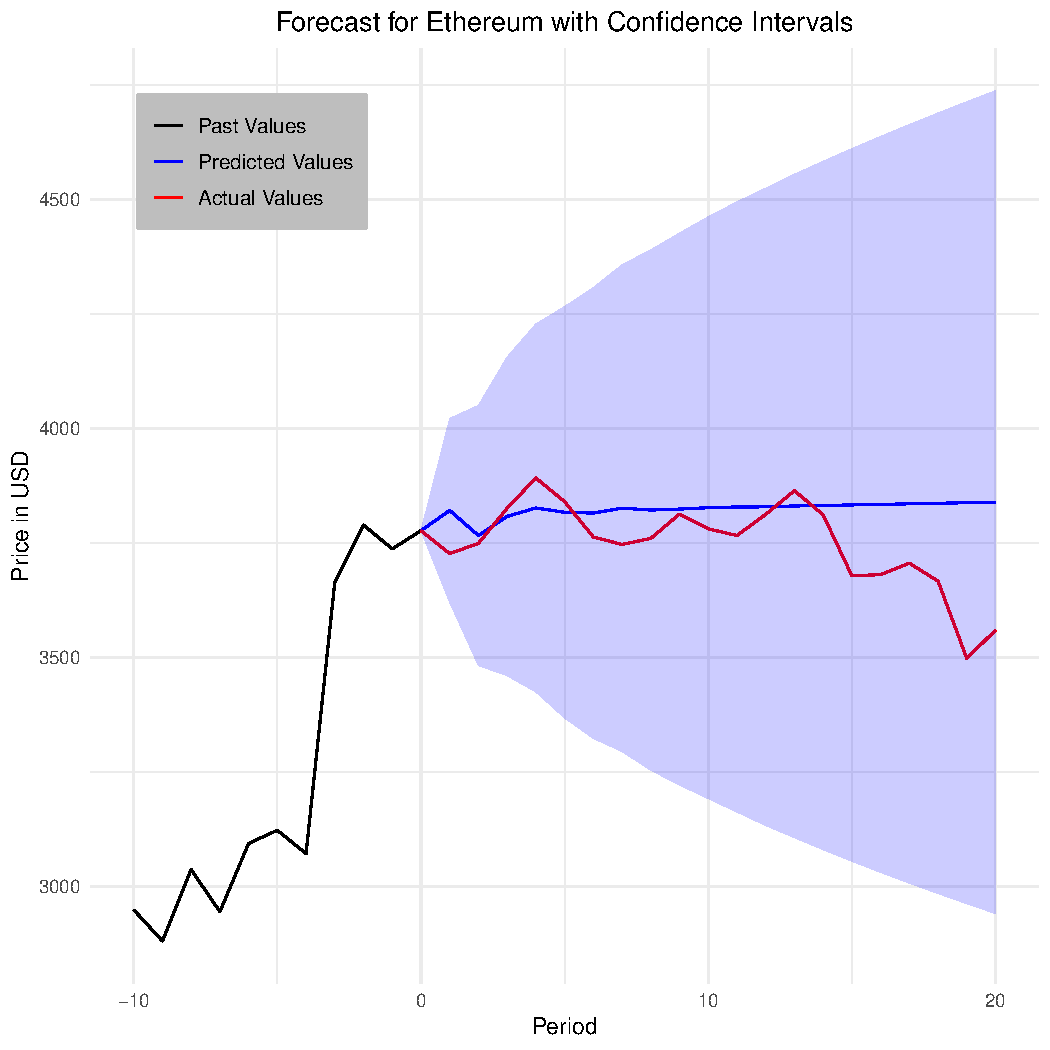
\includegraphics[width=.45\textwidth]{1.Projekt_kode/Billeder/20_day_ahed_Ethereum_from_Solana_Ethereum.pdf}}
  \caption{20-day-ahead prediction plot}
  \label{fig:SOL_ETH_20_DAY_plot}
\end{figure}
\begin{comment}
\begin{center}
    \textbf{ETH \& SOL}
\end{center}

\begin{figure}[H]
  \centering
  \subfloat[][Ethereum]{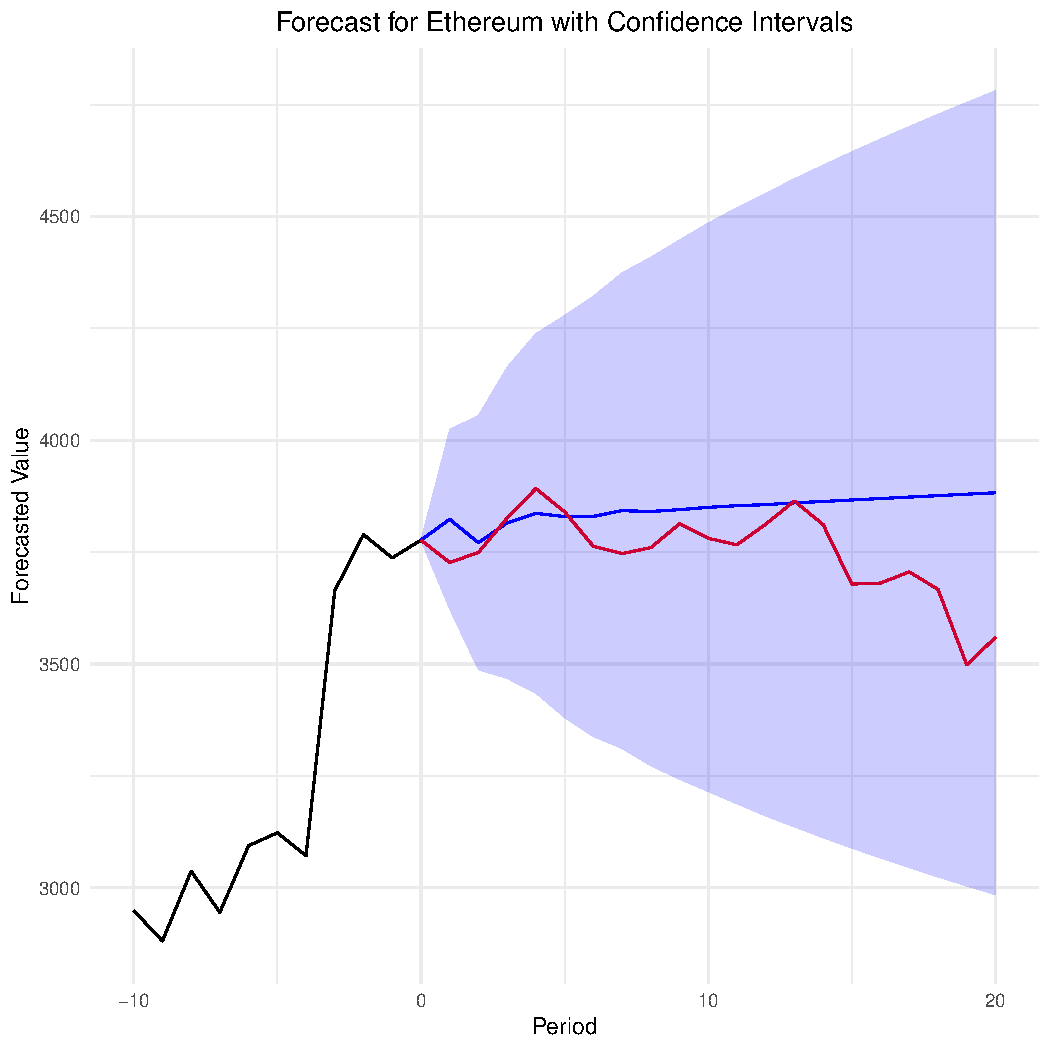
\includegraphics[width=.45\textwidth]{1.Projekt_kode/Billeder/20_day_ahed_Ethereum_from_Ethereum_Solana.pdf}}\quad
  \subfloat[][Solana]{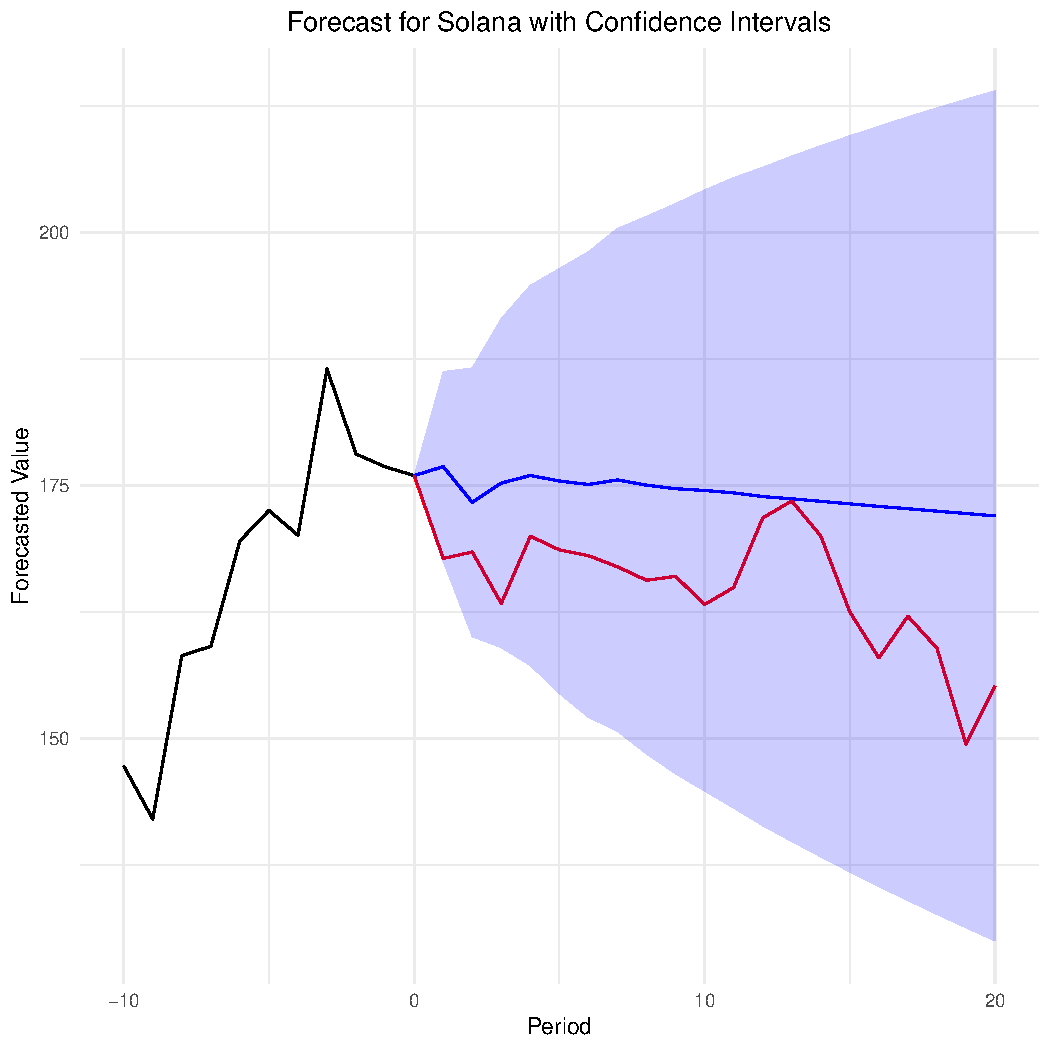
\includegraphics[width=.45\textwidth]{1.Projekt_kode/Billeder/20_day_ahed_Solana_from_Ethereum_Solana.pdf}}
  \label{}
\end{figure}

\end{comment}

\noindent In Figure \ref{fig:SOL_ETH_20_DAY_plot}, the blue line is the predicted prices, the red line is the actual prices, the black line is the actual price before the first prediction, and the shaded area is the $95\%$ confidence interval. The predictions for both SOL and ETH seem to be quite inaccurate. This was to be expected due to cryptocurrencies' high volatility. The predictions for the ETH prices are not catastrophic up until around the 12-days-ahead prediction, where the decrease in price is not caught. Even though this is the case, one could argue that the results are only somewhat accurate since the predictions are close to constant and the actual price fluctuates around this prediction. The reasoning behind the flat predictions could revolve in the model moving towards the long-run equilibrium. It is however positive, that for both graphs the actual values lies within the $95\%$ confidence interval. Below, a table with the model's accuracy measures are stated:

\begin{table}[H]
\centering
\begin{tabular}{lcccccc}
\toprule
\textbf{Metric} & \textbf{One-Day} & \textbf{Two-Day} & \textbf{Three-Day} & \textbf{Four-Day} & \textbf{Five-Day} \\
\midrule
\textbf{MAE} & & & & & \\
Solana        & 28.11133 & 25.22199 & 27.12728 & 27.9634 & 27.72747 \\
Ethereum      & 811.18274 & 771.61202 & 818.57316 & 845.9166 & 847.10831 \\
\midrule
\textbf{RMSE} & & & & & \\
Solana        & 31.24737 & 28.33555 & 30.14608 & 30.94042 & 30.63449 \\
Ethereum      & 953.08236 & 914.34242 & 956.88827 & 979.86588 & 979.72258 \\
\midrule
\textbf{MAPE(\%)} & & & & & \\
Solana        & 19.85790 & 17.85844 & 19.18544 & 19.77437 & 19.62114 \\
Ethereum      & 30.54404 & 29.21761 & 30.93889 & 31.95720 & 32.08274 \\
\bottomrule
\end{tabular}
\caption{Performance Metrics for Solana and Ethereum}
\label{table:SOL_ETH_MAE_RMSE_MAPE}
\end{table}

\noindent  
The MAPE is off by more than $19\%$ and $30\%$ for the one-day-ahead predictions respectively. Furthermore, the prediction accuracy does not seem to deteriorate significantly over five days, and an interesting observation is that all three accuracy measures for SOL are smaller for five-day-ahead compared to the one-day-ahead prediction. The MAPE for SOL indicate that it is somewhat decent. The model's predictability for ETH is more unreliable compared to SOL.
\pause

\subsection{Johansen}
As in Section \ref{englegrangerforecastsection}, we first inspect the 20-day-ahead prediction plots. 
\begin{figure}[H]
  \centering
  \subfloat[][Bitcoin]{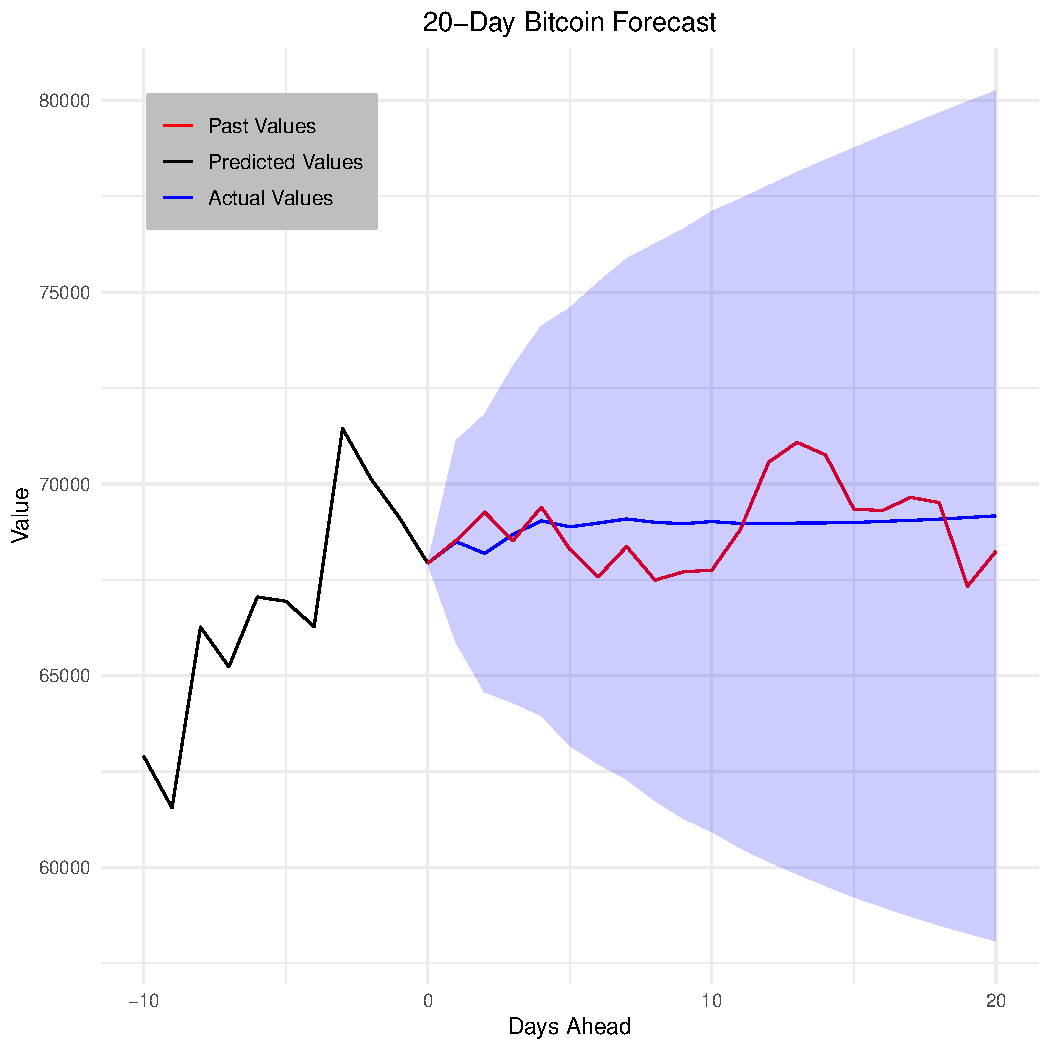
\includegraphics[width=.45\textwidth]{1.Projekt_kode/Billeder/20_day_ahead_Bitcoin_from_johanson.pdf}}\quad
  \subfloat[][Ethereum]{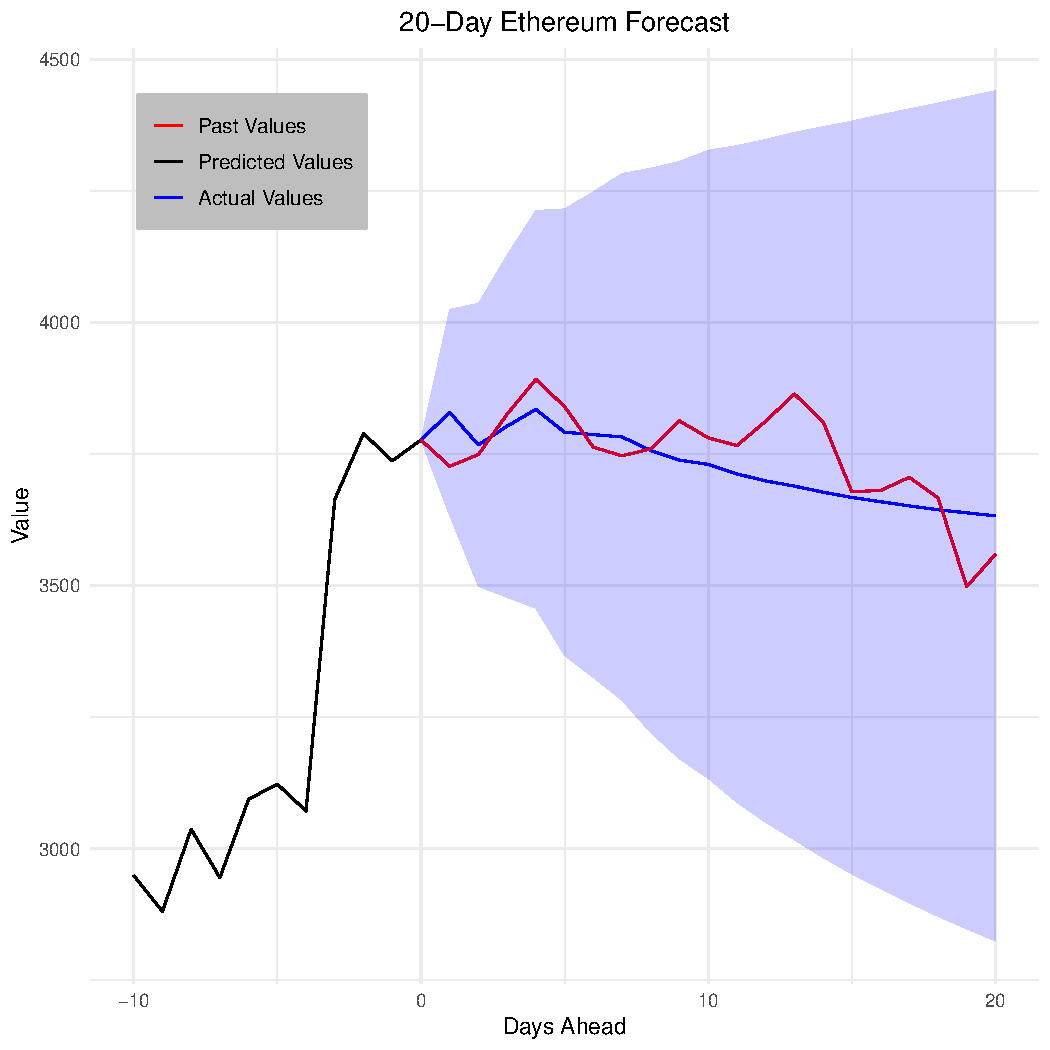
\includegraphics[width=.45\textwidth]{1.Projekt_kode/Billeder/20_day_ahead_Ethereum_from_johanson.pdf}}\\
  \subfloat[][Solana]{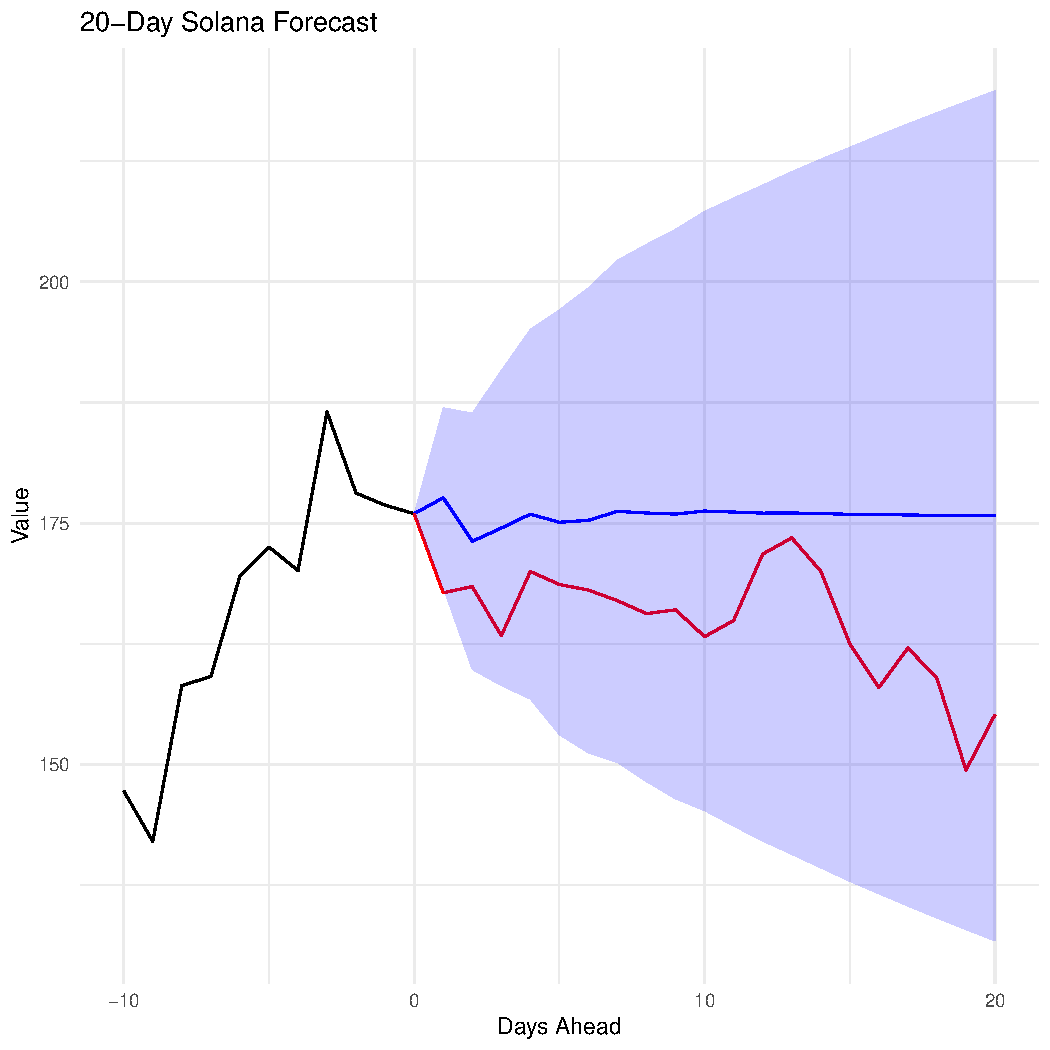
\includegraphics[width=.45\textwidth]{1.Projekt_kode/Billeder/20_day_ahead_Solana_from_johanson.pdf}}\quad
  \subfloat[][Ripple]{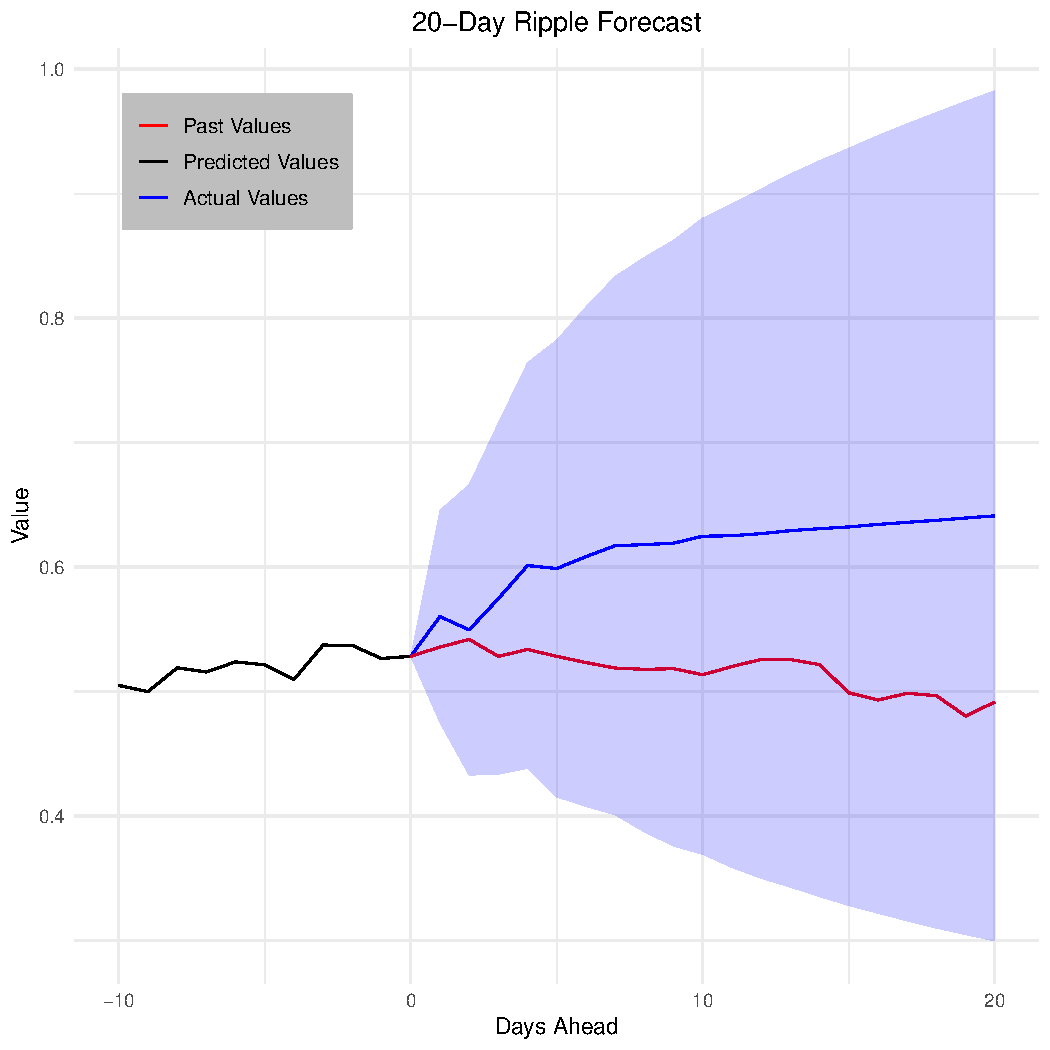
\includegraphics[width=.45\textwidth]{1.Projekt_kode/Billeder/20_day_ahead_Ripple_from_johanson.pdf}}
  \caption{20-day-ahead Predictions}
  \label{fig:20_day_Johansen}
\end{figure}
\noindent The plots seem to be somewhat accurate. All the actual values lies within $95\%$ confidence interval. Furthermore, the model seems to somewhat capture the directional movement initially, especially when looking at BTC and ETH. For BTC the first prediction is so good, that the lines overlap each other.
\begin{table}[H]
\centering
\begin{tabular}{lccccc}
\toprule
\textbf{Metric} & \textbf{One-Day} & \textbf{Two-Day} & \textbf{Three-Day} & \textbf{Four-Day} & \textbf{Five-Day} \\
\midrule
\textbf{MAE} & & & & & \\
Bitcoin   & 436.5510 & 1360.4544 & 2096.0190 & 2372.9510 & 2839.9210 \\
Ethereum  &  29.4897 &   82.8389 &  112.3955 &  128.4171 &  154.1226 \\
Solana    &   5.3342 &    6.5635 &    8.9984 &   11.7554 &   10.2188 \\
Ripple    &   0.0118 &    0.0270 &    0.0461 &    0.0431 &    0.0531 \\
\midrule
\textbf{RMSE} & & & & & \\
Bitcoin   & 514.2976 & 1791.1630 & 2611.2730 & 2950.6350 & 3584.3680 \\
Ethereum  &  36.4638 &  106.7405 &  144.6352 &  162.4643 &  209.4623 \\
Solana    &   5.3489 &    8.0663 &   11.1579 &   14.3040 &   13.0975 \\
Ripple    &   0.0158 &    0.0317 &    0.0529 &    0.0506 &    0.0619 \\
\midrule
\textbf{MAPE} & & & & & \\
Bitcoin   &   0.7173 &    2.2203 &    3.4205 &    3.8782 &    4.6632 \\
Ethereum  &   0.9707 &    2.9081 &    3.9211 &    4.5413 &    5.5665 \\
Solana    &   3.6096 &    4.4267 &    6.0703 &    7.8966 &    6.8306 \\
Ripple    &   2.0972 &    5.1196 &    8.8016 &    8.0928 &   10.1982 \\
\bottomrule
\end{tabular}
\caption{Performance Metrics for Bitcoin, Ethereum, Solana, and Ripple}
\label{fig:johansen_RMSE_MAE_MAPE}
\end{table}
\noindent In the table it can be seen that the MAE gets larger the longer into the future we predict, this is to be expected due to the high volatility of cryptocurrencies. The MAPE especially for one-day-ahead is quint low across the board with Bitcoin standing out as the best, with an prediction error of $0.72$ MAPE and reaching an error at five-day-ahead prediction of $4.66$ MAPE. Just a single prediction namely five-day-ahead for Ripple is larger than $10$ MAPE.\\


\noindent \textbf{Comparison of Engle Granger and Johansen}\\

\noindent First looking at the Figure \ref{fig:20_day_Johansen} and \ref{fig:SOL_ETH_20_DAY_plot}, the predictions looks better for the Johansen model. The Engle Granger and Johansen plots seems to behave somewhat similar, as they capture some movement at the start, and then moves in a straight line, this is expected and it is caused by the error correction.
Secondly, looking at the accuracy measures, it becomes clear that the model build by Johansen compared to the model build by Engle Granger, as all three accuracy measures are significantly lower for the Johansen model than the ones for the Engle Granger model. The MAPE for Johansen only have a single day-ahead prediction which is off by more than $10\%$ and most day-ahead predictions with a deviation from the true value with less than $5\%$. Compared to the Engle Granger, which does not have a single prediction which is off by less than $17\%$. This means the Johansen's worst prediction is better than the Engle Granger's best prediction.\\
It is concluded that the Engle Granger model is somewhat accurate while the Johansen model is quite accurate. Furthermore, we conclude that the Johansen model is the best at forecasting.